\def\duedate{\today}
\def\HWnum{1}
\documentclass[10pt,a4paper]{book}

% custom section formatting
\usepackage{titlesec}
\titleformat{\chapter}[display]
{\normalfont\Large\filcenter\sffamily}
{\titlerule[1pt]%
\vspace{1pt}%
\titlerule
\vspace{1pc}%
\LARGE\MakeUppercase{\chaptertitlename} \thechapter}
{1pc}
{\titlerule
\vspace{1pc}%
\Huge}

% appendix handling
\usepackage[toc,page]{appendix}
    
% encoding for file and font
\usepackage[utf8]{inputenc}
\usepackage[T1]{fontenc}

% math formatting/tools
\usepackage{amsmath}
\usepackage{amssymb}
\usepackage{mathtools}
\usepackage[arrowdel]{physics}

% unit formatting
\usepackage{siunitx}
\AtBeginDocument{\RenewCommandCopy\qty\SI}

% figure formatting/tools
\usepackage{graphicx}
\usepackage{float}
\usepackage{subcaption}
\usepackage{multirow}
\usepackage{import}
\usepackage{pdfpages}
\usepackage{transparent}
\usepackage{currfile}

\NewDocumentCommand\incfig{O{1} m}{
    \def\svgwidth{#1\textwidth}
    \import{./Figures/\currfiledir}{#2.pdf_tex}
}

\newcommand{\bef}{\begin{figure}[h!tb]\centering}
\newcommand{\eef}{\end{figure}}

\newcommand{\bet}{\begin{table}[h!tb]\centering}
\newcommand{\eet}{\end{table}}

% hyperlink references 
\usepackage{hyperref}
\hypersetup{
    colorlinks=true,
    linkcolor=blue,
    filecolor=magenta,
    urlcolor=cyan,
    pdftitle={Physics 1 Notes},
    pdfauthor={Richard Whitehill},
    pdfpagemode=FullScreen
}
\urlstyle{same}

\newcommand{\eref}[1]{Eq.~(\ref{eq:#1})}
\newcommand{\erefs}[2]{Eqs.~(\ref{eq:#1})--(\ref{eq:#2})}

\newcommand{\fref}[1]{Fig.~(\ref{fig:#1})}
\newcommand{\frefs}[2]{Fig.~(\ref{fig:#1})--(\ref{fig:#2})}

\newcommand{\aref}[1]{Appendix~(\ref{app:#1})}
\newcommand{\sref}[1]{Section~(\ref{sec:#1})}
\newcommand{\srefs}[2]{Sections~(\ref{sec:#1})-(\ref{sec:#2})}

\newcommand{\tref}[1]{Table~(\ref{tab:#1})}
\newcommand{\trefs}[2]{Table~(\ref{tab:#1})--(\ref{tab:#2})}

% tcolorbox formatting/definitions
\usepackage[most]{tcolorbox}
\usepackage{xcolor}
\usepackage{xifthen}
\usepackage{parskip}

\definecolor{peach}{rgb}{1.0,0.8,0.64}

\DeclareTColorBox[auto counter, number within=chapter]{defbox}{O{}}{
    enhanced,
    boxrule=0pt,
    frame hidden,
    borderline west={4pt}{0pt}{green!50!black},
    colback=green!5,
    before upper=\textbf{Definition \thetcbcounter \ifthenelse{\isempty{#1}}{}{: #1} \\ },
    sharp corners
}

\newcommand*{\eqbox}{\tcboxmath[
    enhanced,
    colback=black!10!white,
    colframe=black,
    sharp corners,
    size=fbox,
    boxsep=8pt,
    boxrule=1pt
]}

\newtcolorbox[auto counter, number within=chapter]{exbox}{
    parbox=false,
    breakable,
    enhanced,
    sharp corners,
    boxrule=1pt,
    colback=white,
    colframe=black,
    before upper= \textbf{Example \thetcbcounter:}\,,
    before lower= \textbf{Solution:}\,,
    segmentation hidden
}

\newtcolorbox{resbox}{
    enhanced,
    colback=black!10!white,
    colframe=black,
    boxrule=1pt,
    boxsep=0pt,
    top=2pt,
    ams nodisplayskip,
    sharp corners
}


\begin{document}

\prob{1}{
    Consider the scattering of monochromatic photons by free electrons (Compton scattering). \\[3 pt]
    
(a) Assuming that the electron is initially at rest and using energy and momentum conservation, show that the shift in the photon wavelength $\Delta \lambda = \lambda_{f}^{\gamma} - \lambda_{i}^{\gamma}$ is given by
\begin{eqnarray}
    \Delta \lambda = 2 \lambda_{e} \sin^2{\theta_{0}/2}~{\rm with}~\lambda_{e} = \frac{h}{mc}
,\end{eqnarray}
where $m$ is the electron mass, $c$ is the speed of light, and $\theta_0$ is the angle that the momentum of the scattered photon makes with the momentum of the incident photon.
Determine (under the same assumption) the magnitude and direction of the recoil momentum of the electron as a function of the incident-photon energy $E_{i}^{\gamma}$ and scattering angle $\theta_0$.

(b) Assume that the electron has an initial momentum $\va*{p}_{i}$ parallel to the incident-photon momentum $\va*{p}_{i}^{\gamma}$.
Using energy and momentum conservation, show that the wavelength shift is given in this case by
\begin{eqnarray}
    \Delta \lambda = 2 \lambda_{i}^{\gamma} \frac{p_{i}^{\gamma} + p_{i}}{E_{i}/c - p_{i}} \sin^2{\theta/2} 
,\end{eqnarray}
where $\lambda_{i}^{\gamma}$ is the wavelength of the incident photon, $\theta$ is the angle of the scattered photon, and $E_{i} = c^2 \sqrt{p_{i}^2 + (mc)^2}$ is the initial energy of the electron. \\[3 pt]

(c) Show that the result in part (b) above can be derived from the expressions in \\ part (a), where the electron is initially at rest, by a suitable Lorentz transformation.
}

\sol{ 

(a) Consider the reaction $\gamma e \rightarrow \gamma e$ in Fig. \ref{fig:prob1a}.

\begin{figure}[h!tb]
    \centering
    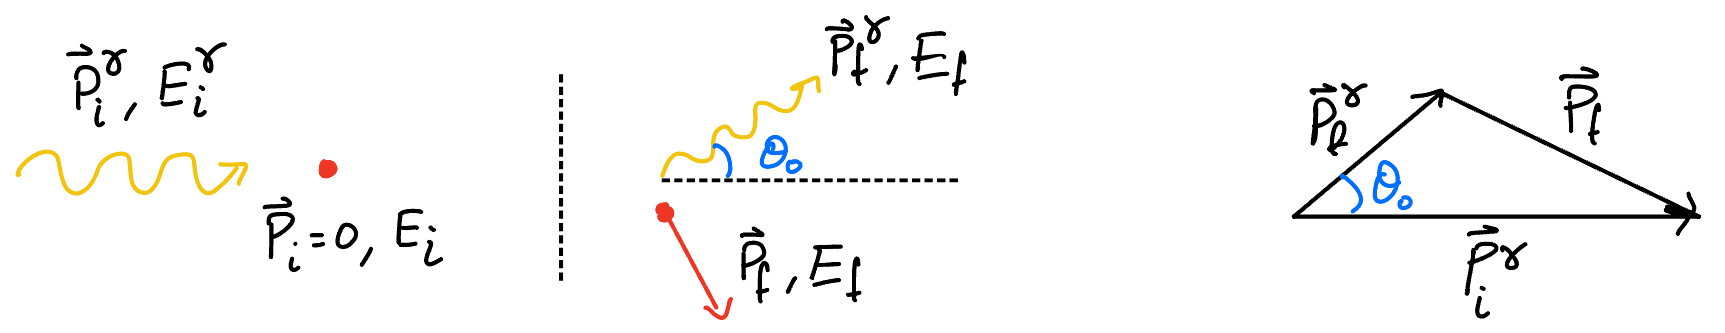
\includegraphics[width=0.7\textwidth]{prob1a.jpeg}
    \label{fig:prob1a}
    \caption{Sketch of the compton scattering process and momentum conservation with electron at rest in the initial state and photon deflecting at angle $\theta_0$ relative to the beam axis.}
\end{figure}

Energy conservation gives that 
\begin{eqnarray}
\label{eq:E-conservation}
    E_{i}^{\gamma} + E_{i} = E_{f}^{\gamma} + E_{f}
.\end{eqnarray}
Note that the energy of the incoming/outgoing photon and electron are given as $E_{i,f}^{\gamma} = p_{i,f}^{\gamma} c$ and $E_{i,f} = c \sqrt{(mc)^2 + p_{i,f}^2}$, respectively.
Using these, Eq. (\ref{eq:E-conservation}) becomes
\begin{eqnarray}
    p_{i}^{\gamma}c + mc^2 = p_{f}^{\gamma}c + c\sqrt{(mc)^2 + p_{f}^2}
.\end{eqnarray}
Dividing through by $c$, subtracting $p_{f}^{\gamma}$ on both sides, and squaring, we obtain
\begin{eqnarray}
    \label{eq:E-conservation-intermediate}
    (m c)^2 + p_{f}^2 = [(p_{i}^{\gamma} - p_{f}^{\gamma}) + mc]^2 = (p_{i}^{\gamma} - p_{f}^{\gamma})^2 + (mc)^2 - 2(p_{i}^{\gamma} - p_{f}^{\gamma}) mc
.\end{eqnarray}

Now, note that momentum conservation tells us that $\va*{p}_{i}^{\gamma} = \va*{p}_{f}^{\gamma} + \va*{p}_{e}'$, and thus,
\begin{eqnarray}
    p_{f}^2 = (\va*{p}_{i}^{\gamma} - \va*{p}_{f}^{\gamma})^2 = (p_{i}^{\gamma})^2 + (p_{f}^{\gamma})^2 - 2 \va*{p}_{i}^{\gamma} \cdot \va*{p}_{f}^{\gamma}
.\end{eqnarray}
Using this, Eq. \ref{eq:E-conservation-intermediate} becomes
\begin{eqnarray}
    - 2 p_{i}^{\gamma} p_{f}^{\gamma} \cos{\theta_0} = -2 p_{i}^{\gamma} p_{f}^{\gamma} - 2 (p_{i}^{\gamma} - p_{f}^{\gamma}) mc
,\end{eqnarray}
and dividing through by $p_{i}^{\gamma} p_{f}^{\gamma}$ after substituting $p_{i,f}^{\gamma} = h/\lambda_{i,f}$ and rearranging we arrive at the desired solution:
\begin{eqnarray}
    \label{eq:1a-result}
    \begin{aligned}
        &\frac{1}{p_{f}^{\gamma}} - \frac{1}{p_{i}^{\gamma}} = \frac{1}{mc}(1 - \cos{\theta_0}) \\
        &\eqbox{ \Delta \lambda = \lambda_{f} - \lambda_{i} = \frac{h}{mc} (1 - \cos{\theta_0}) }
    .\end{aligned}
\end{eqnarray}
Note that $1 - \cos{\theta_0} = 1 - (\cos^2{\theta_0/2} - \sin^2{\theta_0/2}) = 2 \sin^2{\theta_0/2}$.



(b) If the electron is moving collinearly and in the same direction as $\gamma$ before the interaction, energy conservation reads
\begin{eqnarray}
    p_{i}^{\gamma} + \frac{E_{i}}{c} = p_{f}^{\gamma} + \sqrt{(mc)^2 + p_{f}^2}
.\end{eqnarray}

\begin{figure}[h!tb]
    \centering
    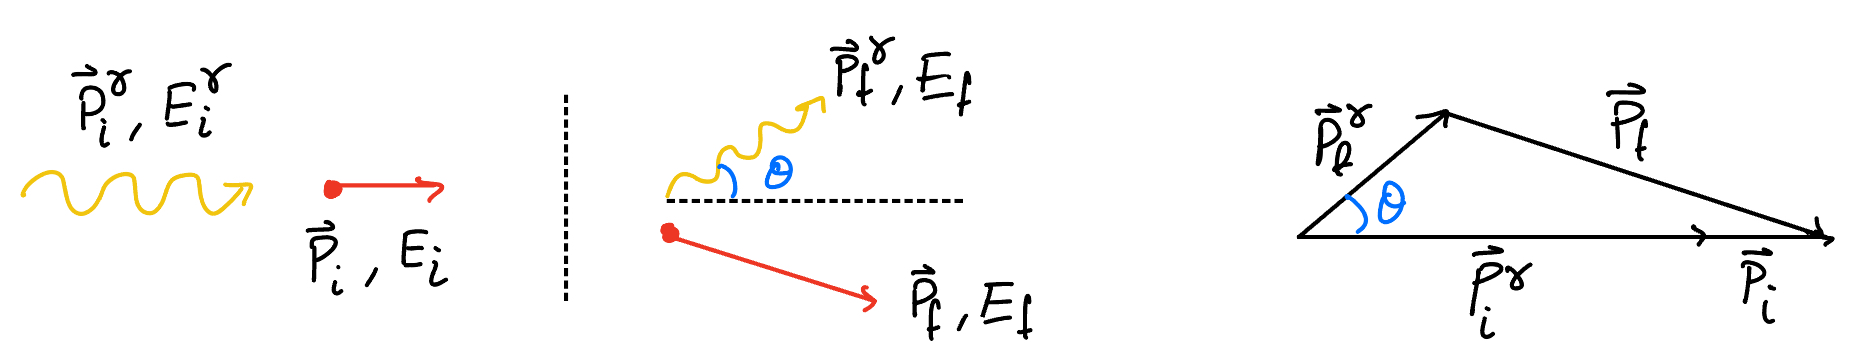
\includegraphics[width=0.7\textwidth]{prob1b.jpeg}
    \label{fig:prob1b}
    \caption{Sketch of compton scattering process with electron with momentum $p_{i}$ in the initial state and photon deflecting at angle $\theta_0$ relative to the beam axis.}
\end{figure}


The manipulations are much the same since $p_{i}$ is a known parameter (and also therefore $E_{i}$).
\begin{eqnarray}
    \label{eq:1b-result}
    \begin{aligned}
        (mc)^2 + p_{f}^2 &= (p_{i}^{\gamma} - p_{f}^{\gamma})^2 + (mc)^2 + p_{i}^2 + 2 \Big( \frac{E_{i}}{c} \Big) (p_{i}^{\gamma} - p_{f}^{\gamma}) \\
        [\va*{p}_{i} + \va*{p}_{i}^{\gamma} - \va*{p}_{f}^{\gamma}]^2 &= (p_{i}^{\gamma} - p_{f}^{\gamma})^2 + p_{i}^2 - 2 \Big( \frac{E_{i}}{c} \Big) (p_{f}^{\gamma} - p_{i}^{\gamma}) \\
        \va*{p}_{i} \cdot \va*{p}_{i}^{\gamma} - \va*{p}_{i} \cdot \va*{p}_{f}^{\gamma} - \va*{p}_{i}^{\gamma} \cdot \va*{p}_{f}^{\gamma} &= - p_{i}^{\gamma} p_{f}^{\gamma} - \frac{E_{i}}{c} (p_{f}^{\gamma} - p_{i}^{\gamma}) \\
        p_{i} p_{i}^{\gamma} - p_{i} p_{f}^{\gamma} \cos{\theta} - p_{i}^{\gamma} p_{f}^{\gamma} \cos{\theta} &= -p_{i} p_{f}^{\gamma} - \frac{E_{i}}{c} (p_{f}^{\gamma} - p_{i}^{\gamma}) \\
        \frac{E_{i}}{c} \Big( \frac{1}{p_{f}^{\gamma}} - \frac{1}{p_{i}^{\gamma}} \Big) &= \frac{p_{i}}{p_{f}^{\gamma}} - \frac{p_{i}}{p_{i}^{\gamma}} + (1 - \cos{\theta}) \\
        \Big( \frac{E_{i}}{c} - p_{i} \Big) \Big( \frac{1}{p_{f}^{\gamma}} - \frac{1}{p_{i}^{\gamma}} \Big) &= 2 \Big( \frac{p_{i}}{p_{i}^{\gamma}} + 1 \Big) \sin^2{\theta/2} \\
        \frac{1}{p_{f}^{\gamma}} - \frac{1}{p_{i}^{\gamma}} &= 2 \Big( \frac{1}{p_{i}^{\gamma}} \Big) \frac{p_{i} + p_{i}^{\gamma}}{E_{i}/c - p_{i}} \sin^2{\theta/2} \\
                                                            &\eqbox{ \Delta \lambda = 2 \lambda_{i}^{\gamma} \frac{p_{i} + p_{i}^{\gamma}}{E_{i}/c - p_{i}} \sin^2{\theta/2} }
    .\end{aligned}
\end{eqnarray}

(c) We can transform from the result Eq. (\ref{eq:1a-result}) in part (a), where the electron is initially at rest, to the result of part (b), given by Eq. (\ref{eq:1b-result}), via a suitable Lorentz transformation.

\begin{figure}[h!tb]
    \centering
    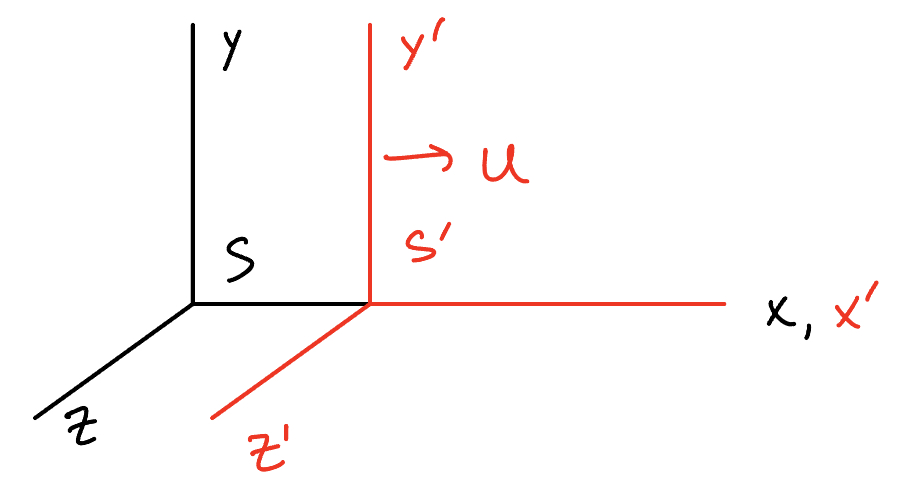
\includegraphics[width=0.5\textwidth]{prob1c.jpeg}
    \label{fig:prob1c}
    \caption{Skeach of Lorentz transformation between frames $S$ and $S'$ moving with relative velocity $u$.}
\end{figure}

Let $S$ be the frame for part (b), where the electron has momentum $p_{i}$ in the initial state, and $S'$ be the frame for part (a), where the electron is at rest in the initial state.
The Lorentz transformation of any 4-vector $a$ from $S'$ to $S$ is given as
\begin{eqnarray}
\label{eq:lorentz-transform}
   \begin{cases}
   c a^{0} = \gamma (c a'^{0} + \beta a'^{x}) \\
   a^{x}  = \gamma (a'^{x} + \beta a'^{0}) \\
   a^{y,z} = a'^{y,z}
   \end{cases} 
.\end{eqnarray}
where the Lorentz factor $\gamma = [1 - \beta^2]^{-1/2}$, where $\beta$ is the velocity of the electron in $S$ (normalized to $c$).
Note that $\gamma^2 = 1 + [p_{i}/(mc)]^2$

Using \eref{lorentz-transform} for the energy of the photon we find
\begin{align}
    \label{eq:initial-transform}
    E_{i}^{\gamma} &= \gamma ( E_{i}'^{\gamma} + \beta p_{i,x}'^{\gamma} ) = \gamma E_{i}'^{\gamma} (1 + \beta) \\
    \label{eq:final-transform}
    E_{f}^{\gamma} &= \gamma E_{f}'^{\gamma} (1 + \beta \cos{\theta_0})
.\end{align}

Now, we can write $E_{i,f}^{\gamma} = c p_{i,f}^{\gamma} = hc/\lambda_{i,f}^{\gamma}$.
Hence, \erefs{initial-transform}{final-transform} tell us how the wavelengths of the initial and final state photon transform between the $S$ and $S'$\footnote{As a sanity check these should reduce to the doppler shift.}:
\begin{align}
    \frac{1}{\lambda_{i}^{\gamma}} &= \frac{\gamma}{\lambda_{i}'^{\gamma}} (1+\beta) \\
    \frac{1}{\lambda_{f}^{\gamma}} &= \frac{\gamma}{\lambda_{f}'^{\gamma}} (1+\beta \cos{\theta_0})
.\end{align}

All that remains is to transform the factor $\cos{\theta_0}$ from $S$ to $S'$.
By definition,
\begin{eqnarray}
    p_{f,x}'^{\gamma} = p_{f}'^{\gamma} \cos{\theta_0} = \frac{E_{f}'^{\gamma}}{c} \cos{\theta_0}
.\end{eqnarray}
Using this equation, we can use the Lorentz transformation to find
\begin{eqnarray}
    \begin{aligned}
        \gamma ( p_{f,x}^{\gamma} - \frac{\beta}{c} E_{f}^{\gamma} ) &= \frac{\gamma E_{f}^{\gamma} ( 1 - \beta \cos{\theta} )}{c} \cos{\theta_0} \\
    \cos{\theta_0} &= \frac{\cos{\theta} - \beta}{1 - \beta \cos{\theta}}
    .\end{aligned}
\end{eqnarray}

Plugging the expressions for $\lambda_{i,f}^{\gamma}$ and $\cos{\theta_0}$ into \eref{1a-result} and allowing a CAS do the algebra we find
\begin{eqnarray}
    \begin{aligned}
        &\gamma \Big[ \lambda_{f}^{\gamma} \Big( 1 + \beta \frac{\cos{\theta} - \beta}{1 - \beta \cos{\theta}} \Big) - \lambda_{i}^{\gamma} (1 + \beta) \Big] = \frac{h}{mc} \Big( 1 - \frac{\cos{\theta} - \beta}{1 - \beta \cos{\theta}} \Big) \\
        &\eqbox{ \Delta \lambda = \frac{p_{i}^{\gamma} + p_{i}}{E_{i}/c - p_{i}} \lambda_{i}^{\gamma} (1 - \cos{\theta}) }
    \end{aligned}
,\end{eqnarray}
as shown in part (b).

}






\prob{2}{
After the discovery of the electron by Thomson in 1897, it was believed that ``atoms were like puddings, with negatively charged electrons stuck in like raisins in a smooth background of positive charge'' (S. Weinberg).
This picture was drastically changed by experiments performed by Rutherford and collaborators, who scattered $\alpha$ particles ($^{4}{\rm He}$ nuclei, which we now know consist of two protons and two neutrons bound together by the nuclear force, having electric charge $2e$) off a thin foil of gold. They observed $\alpha$ particles scattered at large backward angles.
This was totally unexpected, since electrons are much lighter than $\alpha$ particles. \\[3pt]

(a) Consider a particle of mass $M$ and velocity $v$ hitting a particle of mass $m$ at rest and continuing along the same line with velocity $v'$.
Show that, for a given $v$, energy and momentum conservation lead to two possible solutions for $v'$.
If a certain condition is satisfied, one of these solutions corresponds to the case in which particle $M$ inverts its direction of motion.
What is this condition? \\[3pt]

(b) Suppose the $\alpha$ particles (which were in fact emitted by a radium source in Rutherford's experiment) have velocity $v \approx \SI{2.1e9}{\centi\metre\per\second}$, and that the target particles (much heavier than the $\alpha$ particles) have each charge $Ze$.
If the $\alpha$'s and target particles interact via the Coulomb repulsion, what is the distance of closest approach?
Show that this distance is of the order $3Z \times 10^{-14}~\SI{}{\centi\metre}$, and therefore (even for $Z \approx 100$) much smaller than atomic radii.

}

\sol{

(a) This is a simple elastic collision, implying conservation of momentum and kinetic energy.
Momentum conservation give
\begin{eqnarray}
\label{eq:mom-cons}
    Mv = Mv' + mv_{m}
,\end{eqnarray}
and energy conservation gives
\begin{eqnarray} 
\label{eq:kin-cons}
    Mv^2 = Mv'^2 + mv_{m}^2
.\end{eqnarray}
Since we only care about $v'$, we use \eref{mom-cons} to eliminate $v_{m}$ from \eref{kin-cons}
\begin{align}
    v_{m} &= \frac{M}{m} (v - v') \\
    \frac{M^2}{m}(v - v')^2 &= M(v^2 - v'^2)
,\end{align}
and solving the previous equation for $v'$ we find
\begin{eqnarray}
\eqbox{
   v' = 
   \begin{cases}
       v \\
       \frac{M-m}{M+m} v
   .\end{cases}
}
\end{eqnarray}

The first solution implies that no collision occurs, which is in contradiction to our assumption that a collision in fact occurs.
Focusing on the second solution, we see $v' < 0$ (and hence a change of direction for particle $M$) if $m > M$, and furthermore, if $m \gg M$, $v' \approx -v$, which is almost like a "brick wall" scenario.

(b) This problem is one of energy conservation.
The $\alpha$ particles have some initial kinetic energy $T_{i} = m_{\alpha}v^2/2$, and at closest approach $T_{f} = 0$, where
\begin{eqnarray}
    -\frac{1}{2} m_{\alpha} v^2 = -\frac{(2e)(Ze)}{4 \pi \epsilon_0} \frac{1}{r} \Rightarrow \eqbox{ r = \frac{Z e^2}{\pi \epsilon_0 m_{\alpha} v^2} \approx 3Z \times 10^{-14}~\SI{}{\centi\metre}}
,\end{eqnarray}
which is about an order of magnitude (or more) smaller than the typical atomic radii.


}


\prob{3}{

Consider the Rutherford model of the atom: an electron of electric charge $-e$ orbiting a point-like nucleus (much heavier, and hence at rest) of electric charge $Ze$ in a circular orbit of radius $R$.
Knowing that the electron radiates energy away at the rate $\dd{E}/\dd{t}$ given by 
\begin{eqnarray}
    \dv{E}{t} = -\frac{2}{3} \frac{e^2 |\va*{a}(t)|^2}{c^3}
,\end{eqnarray}
where $\va*{a}(t)$ is the acceleration and $c$ is the speed of light, show that it will take a time
\begin{eqnarray}
   \tau = \frac{m^2 c^3}{Z e^{4}} \frac{R^3}{4}
\end{eqnarray}
for the electron to spiral into the nucleus.
Assume that $\tau$ is much larger than the revolution period.
By taking $Z=1$ and $R \approx \SI{1e-8}{\centi\metre}$ appropriate for the hydrogen atom, justify this assumption \textit{a posteriori} by comparing $\tau$ with the revolution period.


}

\sol{

The energy of this system is
\begin{eqnarray}
   E = \frac{1}{2} m v^2 - \frac{Z e^2}{r}
,\end{eqnarray}
when the electron is at a distance $r$ from the nucleus.
Since the acceleration is centripetal\footnote{This is approximately true if we assume that the energy lost per revolution is much smaller than the energy of the system, and thus, that the electron's tangential component of acceleration is very small.} we can write
\begin{eqnarray}
    ma = m\frac{v^2}{r} = \frac{Ze^2}{r^2} \Rightarrow T = \frac{1}{2} V
.\end{eqnarray}
Actually, this is a version of the Virial Theorem for inverse square power laws.
Using this, we find
\begin{eqnarray}
   E = -\frac{1}{2} \frac{Z e^2}{r}
.\end{eqnarray}
From here, we can differentiate this expression of $E$ giving
\begin{eqnarray}
    \dv{E}{t} = \frac{1}{2} \frac{Ze^2}{r^2} \dv{r}{t} = -\frac{2 e^2}{3 c^3} \frac{1}{m^2} \Big( \frac{Ze^2}{r^2} \Big)^2
.\end{eqnarray}
Solving for $\dd{r}/\dd{t}$ gives
\begin{eqnarray}
    \dv{r}{t} = -\frac{4 e^2}{3c^3} \frac{1}{m^2} \frac{Z e ^2}{r^2}
.\end{eqnarray}
We can solve this differential equation as follows
\begin{eqnarray}
    \int_{0}^{\tau} r^{2} \dd{r} = -R^{3} = -\frac{4 Z e^{4}}{m^2 c^3} \tau
.\end{eqnarray}
And finally we rearrange to find 
\begin{eqnarray}
    \eqbox{ \tau = \frac{m^2 c^3}{Z e^{4}} \frac{R^3}{4} \approx Z \times 10^{-10}~{\rm s}}
,\end{eqnarray}
for the conditions stated above.

Note that a distance $R$ from the center one orbital period is
\begin{eqnarray}
    T = 2 \pi \sqrt{ \frac{R^3 m}{Z e ^2}} \approx \frac{1}{\sqrt{Z}} (4 \times 10^{-16}~{\rm s})
,\end{eqnarray}
and hence, the proportion of one period to the time of the electron's orbital decay is given as
\begin{eqnarray}
    \frac{T}{\tau} \approx 4\sqrt{Z} \times 10^{-6}
,\end{eqnarray}
which is quite tiny for any relevant $Z$ and at least tells us that our results are consistent with our assumptions.


}


\prob{4}{

In order to solve the stability problem raised in the previous problem, Niels Bohr proposed in 1913 that the atom can exist only in certain states having energies $E_1 < E_2 < \ldots$, that is, atomic energies are quantized.
To obtain these energies, Bohr assumed that the angular momentum of an electron of mass $m$ and electric charge $-e$ in a \textit{stable circuilar orbit} of radius $r$ around a nucleus of eletric charge $Ze$ is an integer multiple $n$ of the Planck constant $\hbar = h/(2 \pi)$.
Following Bohr, calculate the energies $E_{n}$.

}

\sol{

In the previous problem, we saw that for an electron in circular orbit about the nucleus that
\begin{eqnarray}
   E = -\frac{1}{2} \frac{Z e^2}{r}
.\end{eqnarray}
Since the angular momentum is postulated to be
\begin{eqnarray}
   L = m r v = \sqrt{(Z e^2)mr} = n \hbar \Rightarrow r = \frac{n^2 \hbar^2}{(Z e^2) m}
.\end{eqnarray}
Substituting into our expression for the energy of the system, we have the ``quantized energy levels'' to be
\begin{eqnarray}
    E_{n} = -\frac{(Z e^2)^2 m}{2 n^2 \hbar^2} \approx -13.6~{\rm eV} \times \frac{Z^2}{n^2}
.\end{eqnarray}


}


\prob{5}{

In the old quantum theory, one assumes that the particles follow the laws of classical mechanics, but postulates further that, of all the solutions of the equations of motion, one must only retain those which satisfy certain \textit{ad hoc} quantization rules.
One therefore selects a discontinuous family of motions; these are, by hypothesis, the only motions which are realized in nature.
The discontinuous sequence of energy values thus obtained constitutes the spectrum of quantized energy levels. \\[3pt]

For a one dimensional periodic motion, the quantization rule -- known as the Bohr-Sommerfield quantization rule -- is
\begin{eqnarray}
    \oint_{E} \dd{q} p = n h \quad n = 1,2,\ldots
,\end{eqnarray}
where $h$ is Planck's constant and the symbol $\oint_{E}$ means that one must integrate over a complete period of the motion corresponding to the energy $E$.
Here $q$ and $p$ are the position and momentum variables, respectively.
The integral is known as the action integral.
Apply this rule to the case of the one-dimensional harmonic oscillator for which
\begin{eqnarray}
   E = \frac{p^2}{2m} + \frac{m \omega^2}{2} q^2 
.\end{eqnarray}
Calculate the energy, period, and amplitude of the quantized trajectories.

}

\sol{

For this problem, the quantization condition reads
\begin{eqnarray}
    2 \int_{-\sqrt{2E/m\omega^2}}^{\sqrt{2E/m\omega^2}} \dd{q} \sqrt{2 m E - m^2 \omega^2 q^2} = \frac{2 \pi E}{\omega} = nh \Rightarrow \eqbox{ E_{n} = n \hbar \omega}
.\end{eqnarray}
The period of the motion is simply $2 \pi / \omega$ and the amplitude of the motion is found as follows
\begin{eqnarray}
    E_{n} = \frac{1}{2} m \dot{q}^2 + \frac{1}{2} m \omega^2 q^2
.\end{eqnarray}
Since the classical solution for the harmonic oscillator is $q = A \cos{(\omega t - \varphi)}$, we have
\begin{eqnarray}
    \eqbox{ A_{n} = \sqrt{ \frac{ 2 n \hbar \omega }{m \omega^2} } = \sqrt{ \frac{2 \hbar}{m \omega} n } }
.\end{eqnarray}


}


\prob{6}{

Quantize the \textit{circular} electronic orbits of the hydrogen atom by applying the Bohr-Sommerfield rule introduced in the previous problem.
Determine the energy, period, and radius of the quantized orbits.
Calculate specifically the numerical values of the energy, period, and radius of the lowest orbit.
Use $mc^2 \approx \SI{0.51e6}{\eV}$ and $\hbar c / e^2 \approx 137$.

}

\sol{

From problem 4, we can write the energy of the hydrogen atom as 
\begin{eqnarray}
   E = -\frac{p^2}{2m} \Rightarrow p = \sqrt{-2mE}
.\end{eqnarray}
Since the momentum is constant for a given orbit, the Bohr-Sommerfield quantization rule gives
\begin{eqnarray}
 2 \pi r p = n h \Rightarrow L = n \hbar
.\end{eqnarray}
This is exactly the postulated angular momentum for the Bohr model of the atom, meaning
\begin{eqnarray}
    \eqbox{ E_{n} = -\frac{m (Z e^2)^2}{2 \hbar^2} \frac{1}{n^2} = -\frac{E_0 \alpha^2}{2} \frac{Z^2}{n^2} \approx -13.6~{\rm eV} \times \frac{Z^2}{n^2}}
,\end{eqnarray}
and furthermore, 
\begin{eqnarray}
    r_{n} = -\frac{Z e^2}{2 E_{n}} = \frac{e^2}{m c^2 \alpha^2} \frac{n^2}{Z} \approx (0.53 \times 10^{-8}~{\rm cm}) \frac{n^2}{Z}
.\end{eqnarray}
Note that the factor in front of the $n^2/Z$ is the Bohr radius, which is the most probable distance for the electron from the nucleus.
Finally, the period of motion is
\begin{eqnarray}
    \begin{aligned}
        T_{n} &= 2 \pi \frac{r_{n}}{v_{n}} = 2 \pi r_{n} \frac{m r_{n}}{L_{n}} = \frac{2 \pi m}{n \hbar} \Big( \frac{a_0 n^2}{Z} \Big)^2 = \frac{2 \pi m a_0^2}{\hbar} \frac{n^3}{Z^2} \\
              &= \eqbox{\frac{2 \pi a_0}{\alpha c} \frac{n^3}{Z^2} \approx (1.5 \times 10^{-16}~{\rm s}) \frac{n^3}{Z^2} }
    \end{aligned}
.\end{eqnarray}




}


\prob{7}{

In addition to its failures in explaining the blackbody radiation spectrum, the photo-electric effect, and the stability of atoms and spectral lines, classical physics could also not explain the heat capacity of a solid. \\[3pt]

(a) Assume a solid of volume $V$ with $N$ atoms (or molecules) can be modeled as a set of $3N$ independent one-dimensional harmonic oscillators of frequency $\nu_0$ (that is, all oscillators have the same frequency $\nu_0$).
Making use of the equipartition theorem, calculate the total average energy $E$ of the solid at temperature $T$ and derive the Dulong-Petit law for the heat capacity (at constant volume)
\begin{eqnarray}
    c_{V} = \Big( \pdv{E}{T} \Big)_{V} = 3 N k_{B}
,\end{eqnarray}
where $k_{B}$ is the Boltzmann's constant. \\[3pt]

(b) The observed heat capacity of a solid is not a constant independent of $T$, but rather vanishes as $T^3$ at low temperature and approaches the classical prediction (the Dulong-Petit law) at high temperature.
Einstein (1907) proposed that the energy of each harmonic oscillator is quantized and that its average energy at temperature $T$ is given by
\begin{eqnarray}
    \expval{E} = \frac{h \nu_0}{\exp(h \nu_0/k_{B}T) - 1}
,\end{eqnarray}
see class notes.
Show that the heat capacity is now found to be
\begin{eqnarray}
    c_{V} = 3 N k_{B} \frac{x_0^2 e^{x_0}}{(e^{x_0}-1)^2}, \quad x_0 = \frac{h \nu_0}{k_{B} T}
.\end{eqnarray}
Does $c_{V}$ vanish as $T \rightarrow 0$?
What happens at high temperature? \\[3pt]

(c) Einstein's theory predicts that $c_{V}$ vanishes exponentially at low temperature, a result that is at variance with experimental observations.
A more realistic model of a solid is that it consists of $3N$ independent harmonic oscillators (modes) with a distribution in frequency $g(\nu)$ given by
\begin{eqnarray}
    g(\nu) = 4\pi \frac{V}{v_{S}^3} \nu^2
,\end{eqnarray}
where $v_{S}$ is the sound velocity in the solid, such that 
\begin{eqnarray}
    {\rm number~of~modes} = \int_{0}^{\nu_{\rm max}} \dd{\nu} g(\nu) = 3N
.\end{eqnarray}
This condition fixes $\nu_{\rm max}$ as a function of the density $N/V$.
Introduce the parameter $T_{D}$ (the Debye temperature) defined as $T_{D} = h \nu_{\rm max}/k_{B}$ and show that the total average energy at temperature $T$ is given by
\begin{eqnarray}
    E = 9 N h \nu_{\rm max} \Big( \frac{T}{T_{D}} \Big)^{4} \int_{0}^{T_{D}/T} \dd{x} \frac{x^3}{e^{x} - 1}
,\end{eqnarray}
and that the constant-volume heat capacity is proportional to $T^3$ for low $T$, in agreement with experiment.
Show that it also satisfies the Dulong-Petit law at high temperatures.

}


\sol{

(a) The Hamiltonian for a 1D harmonic oscillator is given by
\begin{eqnarray}
   H = \frac{p^2}{2m} + \frac{m \omega_0^2}{2} q^2 
,\end{eqnarray}
where $p$ and $q$ are the generalized momentum and spatial variables of the oscillator and $\omega_0 = 2 \pi \nu_{0}$ is the angular frequency of the oscillator.
The equipartition theorem states that for a system
\begin{eqnarray}
   E = \sum_{\rm particles} \sum_{\rm d.o.f.} \frac{1}{2} k_{B} T = 3 N k_{B} T
.\end{eqnarray}
From this, the heat capacity of a solid modeled in this way is
\begin{eqnarray}
    \eqbox{ c_{V} = \Big( \pdv{E}{T} \Big)_{V} = 3 N k_{B} }
,\end{eqnarray}
which is constant with temperature.

(b) We can derive the average energy for an oscillator at temperature $T$ using some basic results from statistical mechanics.
Namely, the energy of an ensemble is given by
\begin{eqnarray}
    \expval{E} = -\frac{1}{\cal Z} \pdv{Z}{\beta} = -\pdv{\ln{\cal Z}}{\beta}
,\end{eqnarray}
where $\cal Z$ is the partition function of our ensemble and defined as
\begin{eqnarray}
    {\cal Z} = \sum_{i} e^{-\beta E_{i}}
,\end{eqnarray}
where $\beta^{-1} = k_{B}T$.
In our case, the energy of an oscillator with frequency $\nu_0$ is quantized (per Einstein's postulate) as $E_{n} = n h \nu_0$.
Putting this into the partition function definition, we find
\begin{eqnarray}
    {\cal Z} = \sum_{n} (e^{- \beta h \nu_0})^{n} = \frac{1}{1 - e^{-\beta h \nu_0}}
.\end{eqnarray}
Hence, the average energy of an oscillator is 
\begin{eqnarray}
    \begin{aligned}
        \expval{E} &= - (1 - e^{-\beta h \nu_0}) \pdv{\beta} \Big[ \frac{1}{1 - e^{-\beta h \nu_0}} \Big] \\
                   &= -(1 - e^{-\beta h \nu_0}) [-(1 - e^{-\beta h \nu_0})^{-2} (h \nu_0) e^{-\beta h \nu_0}] \\
                   &= \frac{h \nu_0}{e^{\beta h \nu_0} - 1}
    \end{aligned}
,\end{eqnarray}
which is the result quoted above.

Now, we can derive the heat capacity of a solid by setting the energy of the solid to be $E = 3 N \expval{E_{\rm o}}$.
Then
\begin{eqnarray}
    \begin{aligned}
        c_{V} &= 3N \Big( \pdv{\expval{E}}{T} \Big)_{V} = 3N \Big( -\frac{\beta^2}{k_{B}} \Big) \pdv{\expval{E}}{\beta} \\
              &= \frac{3 N \beta^2}{k_{B}} \frac{(h \nu_0)^2 e^{\beta h \nu_0}}{(e^{\beta h \nu_0} - 1)^2}
    .\end{aligned}
\end{eqnarray}
If we rewrite our result in terms of the dimensionless variable $x_0 = \beta h \nu_0$, we have
\begin{eqnarray}
    \eqbox{ c_{V} = \frac{3N}{k_{B}} \frac{x_0^2 e^{x_0}}{(e^{x_0} - 1)^2} }
.\end{eqnarray}
From this expression, we can evaluate the extreme behavior of this function.
First, as $T \rightarrow 0$, $x_0 \rightarrow \infty$ and $c_{V} \rightarrow 0$ since the term $e^{2x_0}$ in the denominator dominates the expression at large $x_0$, meaning that $c_{V}$ vanishes exponentially fast at small temperatures.
Additionally, for large temperatures $T$ (and thus $x_0 \approx 0$), we find
\begin{eqnarray}
    c_{V} = 1 - \frac{x_0^2}{12} + {\cal O}(x_0^{4}) \rightarrow 1 ~{\rm as}~ T \rightarrow \infty
.\end{eqnarray}

(c) To correct Einstein's prediction, we allow the modes to oscillate at independent frequencies $\nu \in [0,\nu_{\rm max}]$ with a distribution $g(\nu) = 4 \pi (V/v_{S}^3) \nu^2$.
We can solve for $\nu_{\rm max}$ as follows:
\begin{eqnarray}
    4 \pi \frac{V}{v_{S}^3} \int_{0}^{\nu_{\rm max}} \dd{\nu} \nu^2 = \frac{4 \pi}{3} \frac{V}{v_{S}^3} \nu_{\rm max}^3 = 3 N \Rightarrow \nu_{\rm max} = \Big[ \frac{9}{4 \pi} \Big( \frac{N}{V} \Big) \Big]^{1/3} v_{S}
.\end{eqnarray}
At this point, the average energy of the solid is given simply as 
\begin{eqnarray}
    E = \int_{0}^{\nu_{\rm max}} g(\nu) \frac{h \nu}{e^{\beta h \nu} - 1} \dd{\nu}
.\end{eqnarray}
Switching to a dimensionless integration variable $x = \beta h \nu$ we find
\begin{eqnarray}
    \begin{aligned}
        E &= \frac{9 N}{\nu_{\rm max}^3} \int_{0}^{T_{D}/T} \Big( \frac{x}{\beta h} \Big)^2 \frac{1}{\beta} \frac{x}{e^{x} - 1} \Big( \frac{1}{\beta h} \Big) \dd{x} \\
          &= \frac{9 N}{\nu_{\rm max}^3 \beta^{4} h^3} \int_{0}^{T_{D}/T} \frac{x^3}{e^{x}-1} \dd{x} \\
          &= 9 N h \nu_{\rm max} \Big( \frac{1}{\beta h \nu_{\rm max}} \Big)^{4} \int_{0}^{T_{D}/T} \frac{x^3}{e^{x} - 1} \dd{x} \\
          &= \eqbox{9 N h \nu_{\rm max} \Big( \frac{T}{T_{D}} \Big)^{4} \int_{0}^{T_{D}/T} \frac{x^3}{e^{x} - 1} \dd{x} }
    \end{aligned}
,\end{eqnarray}
where we have expressed $\nu_{\rm max}$ in terms of $T_{D}$ and $g(\nu) = 9 N \nu^2 / \nu_{\rm max}^3$.

Let us now evaluate the behavior of $c_{V}$ for extreme temperatures

Now, the heat capacity of the solid is given as
\begin{eqnarray}
    c_{V} = 9 N h \nu_{\rm max} \pdv{T} \Bigg[ \Big( \frac{T}{T_{D}} \Big)^{4} \int_{0}^{T_{D}/T}\frac{x^3}{e^{x} - 1} \dd{x} \Bigg]
.\end{eqnarray}
Note that the physics is contained in the derivative of the factor in brackets, so for our analysis we only consider this term, which we denote $\tilde{c}_{V}$.
Carrying out the arithmetic, we have 
\begin{eqnarray}
   \begin{aligned}
       \tilde{c}_{V} &= \frac{4}{T_{D}} \Big( \frac{T}{T_{D}} \Big)^{3} \int_{0}^{T_{D}/T} \frac{x^3}{e^{x} - 1} \dd{x} + \Big( \frac{T}{T_{D}} \Big)^{4} \Big( -\frac{T_{D}}{T^2} \Big) \frac{(T_{D}/T)^3}{e^{T_{D}/T} - 1} \\
                     &= T^3 \Bigg[ \frac{4}{T_{D}^{4}} \int_{0}^{T_{D}/T} \frac{x^{3}}{e^{x} - 1} \dd{x} - \frac{1}{T^{4}(e^{T_{D}/T} - 1)} \Bigg]
   \end{aligned} 
.\end{eqnarray}
If we consider $T \rightarrow 0$, then
\begin{eqnarray}
    \eqbox{ \tilde{c}_{V} \approx T^3 \Bigg[ \frac{4}{T_{D}^{4}} \int_{0}^{\infty} \frac{x^3}{e^{x} - 1} \dd{x} \Bigg] }
,\end{eqnarray}
which has the desired behavior.

At large temperatures (i.e. $T \rightarrow \infty$), we have
\begin{eqnarray}
    \begin{aligned}
        \tilde{c}_{V} &\approx \frac{4T^3}{T_{D}^{4}} \int_{0}^{T_{D}/T} [x^2 + {\cal O}(x^3)] \dd{x} - \frac{1}{T[ (1 + T_{D}/T + {\cal O}(T_{D}^2/T^2)) - 1 ]} \\
                      &\approx \frac{4}{3 T_{D}} - \frac{1}{T_{D}} = \frac{1}{3 T_{D}} = \frac{1}{3} \frac{k_{B}}{h \nu_{\rm max}}
    \end{aligned}
,\end{eqnarray}
and therefore
\begin{eqnarray}
    \eqbox{ c_{V} = 3 N k_{B} }
.\end{eqnarray}

\textit{ In hindsight, it may be simpler to define $\tilde{E} = E/(9 N h \nu_{\rm max})$, consider the limiting behavior of $\tilde{E}(T)$, and let $\tilde{c}_{V} = (\partial_{T} \tilde{E})_{V}$.
From this approach, we only have to keep track of one term instead of two, which is certainly cleaner. }


}






\end{document}
